\documentclass[a4paper,10pt]{article}
% \documentclass[a4paper,10pt,draft]{article}  % DEBUG boxes

%A Few Useful Packages
\usepackage{marvosym}
\usepackage{fontspec} 					%for loading fonts
\usepackage{xunicode,xltxtra,url,parskip} 	%other packages for formatting
\RequirePackage{color,graphicx}
\usepackage[usenames,dvipsnames]{xcolor}
\usepackage{fullpage}
\usepackage{supertabular} 				%for Grades
\usepackage{titlesec}					%custom \section
\usepackage{wasysym}
\usepackage{multirow}
\usepackage{graphicx}
\graphicspath{ {./../public/} }

%Setup hyperref package, and colours for links
\usepackage{hyperref}
\definecolor{linkcolour}{rgb}{0,0.2,0.6}
\hypersetup{colorlinks,breaklinks,urlcolor=linkcolour, linkcolor=linkcolour}

%FONTS
% \defaultfontfeatures{Mapping=tex-text}
%\setmainfont[SmallCapsFont = Fontin SmallCaps]{Fontin}
%%% modified for Karol Kozioł for ShareLaTeX use
% \setmainfont[
% SmallCapsFont = Fontin-SmallCaps.otf,
% BoldFont = Fontin-Bold.otf,
% ItalicFont = Fontin-Italic.otf
% ]
% {Fontin.otf}
%%%

%CV Sections inspired by:
%http://stefano.italians.nl/archives/26
\titleformat{\section}{\Large\scshape\raggedright}{}{0em}{}[\titlerule]
\titlespacing{\section}{0pt}{3pt}{3pt}
%Tweak a bit the top margin
\addtolength{\voffset}{-1.3cm}

%Italian hyphenation for the word: ''corporations''
% \hyphenation{im-pre-se}

%-------------WATERMARK TEST [**not part of a CV**]---------------
\usepackage[absolute]{textpos}

\setlength{\TPHorizModule}{30mm}
\setlength{\TPVertModule}{\TPHorizModule}
\textblockorigin{2mm}{0.65\paperheight}
\setlength{\parindent}{0pt}

%--------------------BEGIN DOCUMENT----------------------
\begin{document}

\pagestyle{empty} % non-numbered pages

\font\fb=''[cmr10]'' %for use with \LaTeX command

%--------------------TITLE-------------
\par{\centering
		{\Huge Sindri \textsc{Guðmundsson}
	}\bigskip\par}

%--------------------SECTIONS-----------------------------------
%Section: Personal Data
\section{Personal Data}

\begin{tabular}{rlr}
    \textsc{Place and Date of Birth:} & Iceland | 25 September 1988
    &\multirow{9}{*}{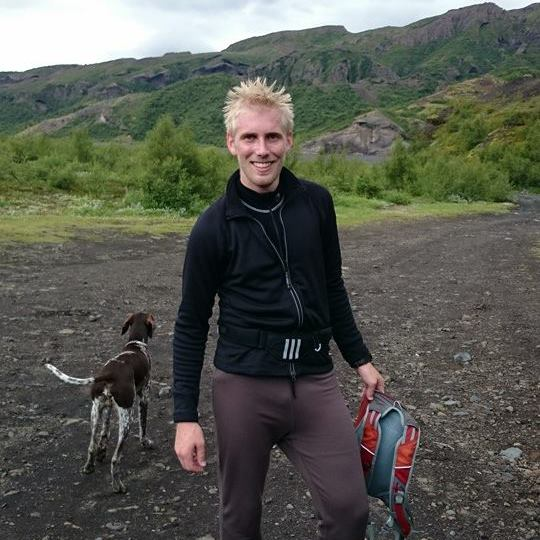
\includegraphics[scale=0.18]{sindri}}\\
    \textsc{Location:}   & Reykjavík, Iceland \\
    \textsc{email:}     & \href{mailto:sindrigudmundsson@gmail.com}{sindrigudmundsson@gmail.com}\\
    \textsc{homepage:}     & \href{https://irdn.is}{irdn.is} \\
    \textsc{github:}     & \href{https://github.com/sindrig}{/sindrig} \\
    \multicolumn{3}{c}{} \\
    \multicolumn{3}{c}{} \\
    \multicolumn{3}{c}{} \\
    \multicolumn{3}{c}{} \\
\end{tabular}


%Section: Work Experience at the top
\section{Work Experience}
\begin{tabular}{r|p{10cm}}
 \emph{Current} & Chief Technology Officer at \href{www.aftra.io}{Aftra}, Reykjavík \\\textsc{Jun 2024}&\footnotesize{Developer/DevOps/Platform engineer/Manager}\\\multicolumn{2}{c}{} \\
 \textsc{Dec 2021-Jun 2024} & Developer at \href{www.syndis.is}{Syndis}, Reykjavík \\&\footnotesize{Developer/DevOps/Platform engineer}\\\multicolumn{2}{c}{} \\
 \textsc{Aug 2020-Nov 2021} & Devops \& AWS specialist at \href{www.andes.is}{Andes}, Reykjavík \\&\footnotesize{DevOps/Platform engineer \& AWS specialist}\\\multicolumn{2}{c}{} \\
 \textsc{Jan 2016-Sep 2020} & Software developer at \href{www.tempo.io}{Tempo}, Reykjavík \\&\footnotesize{Mostly platform/dev-ops but worked on everything from writing front-end in React.js to back-end in python/java to ops/dev-ops mostly with python+aws.}\\\multicolumn{2}{c}{} \\

 \textsc{Nov 2010-Apr 2020} & Developer at \href{www.hreyfistjornun.is}{Hreyfistjórnun}, Reykjavík \\&\footnotesize{Wrote a web application using Ruby on Rails for physiotherapists and patients to communicate and record physical exercise. Rewrote the
system in 2013 using Python/Django.}\\
& \footnotesize{Also wrote a VOIP client using Asterisk and Python.}\\
& \footnotesize{Played a role in the introduction of physical exercise
prescriptions by the government.}\\\multicolumn{2}{c}{} \\

 \textsc{Mar 2011-Jan 2016} & Software developer at \href{www.trackwell.com}{Trackwell}, Reykjavík \\&\footnotesize{Rewrote large parts of \href{www.timon.is}{Tímon} using Python\&Django. Also worked on multiple other projects using various tools.}\\\multicolumn{2}{c}{} \\

 \textsc{Jan 2012-May 2012} & Assistant teacher at \href{www.hi.is}{The University of Iceland}, Reykjavík \\&\footnotesize{Software development (Þróun hugbúnaðar) assistant teacher spring 2012.}\\\multicolumn{2}{c}{} \\

 \textsc{Sep 2001-May 2011} & Football coach at \href{www.vikingur.is}{Víkingur FC}, Reykjavík \\&\footnotesize{Youth football (soccer) coach. Mostly U12 and U16 boys.}\\\multicolumn{2}{c}{} \\

 \end{tabular}

%Section: Education
\section{Education}
\begin{tabular}{rl}
 \textsc{June} 2012 & Bachelor of Science in \textsc{Computer Science}\\&\textbf{University of Iceland}, Reykjavík\\
&\normalsize \textsc{Final grade}: 8.9\\&\\

 \textsc{June} 2008 & Undergraduate degree\\&\textbf{The commercial college of Iceland}, Reykjavík
\end{tabular}

%Section: Certificates and additional info
\section{Certificates}
\begin{tabular}{rl}
    & \href{https://aws.amazon.com/certification/certified-developer-associate/}{AWS Certified Developer - Associate}\\
    & \href{https://aws.amazon.com/certification/certified-solutions-architect-associate/}{AWS Certified Solutions Architect - Associate}
\end{tabular}



\section{Social Activities}
\begin{tabular}{r|p{10cm}}

 \textsc{Jan 2018-Feb 2019} & Board member at \href{www.vikingur.is}{Víkingur FC} (football dept.), Reykjavík \\\multicolumn{2}{c}{} \\

 \textsc{June 2011-Jan 2018} & Board member at Berserkir FC, Reykjavík \\\multicolumn{2}{c}{} \\

\end{tabular}
%Section: Languages
\section{Languages}
\begin{tabular}{rl}
 \textsc{Icelandic:}&Mothertongue\\
\textsc{English:}&Fluent\\
\textsc{Danish:}&Basic Knowledge\\
\textsc{French:}&Very Limited Knowledge\\
\end{tabular}

\section{Interests and Activities}
Technology, Open-Source, Programming,\\
Running, Football, Camping, Hiking, Hunting, Skiing

\end{document}
